\icode{E-MI-MU-L3-261104-002}
（多选）
如图所示，穿过光滑动滑轮的轻绳两端分别固定在\(M\)、\(N\)两点，质量为\(m\)的物块通过轻绳拴接在动滑轮的轴上，给物块施加一个水平向左的拉力\(F\)，系统静止平衡时，滑轮到固定点\(M\)、\(N\)的两部分轻绳与水平方向的夹角分别为\qty{53}{\degree}和\qty{37}{\degree}，滑轮质量忽略不计，重力加速度为\(g\)，\(\sin\)\qty{37}{\degree}=0.6，\(\sin\)\qty{53}{\degree}=0.8。下列说法正确的是\paren[]

	
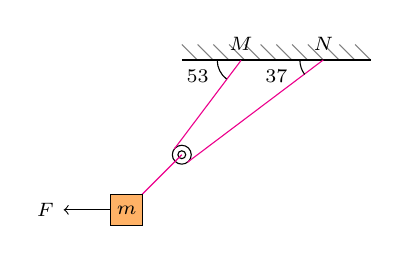
\begin{tikzpicture}[font=\scriptsize]
	\foreach \x in {0,.2,...,2.2}
		\draw[gray] (\x,1.4)--++(.2,-.2);
	\draw[thick] (0,1.2)--(2.4,1.2);
	\draw[fill=white] (0,0) circle(.12) (0,0) circle(.05);
	\draw[->] (-.9,-.7)--(-1.5,-.7)node[left]{\(F\)};
	\draw[magenta] (-53:.12)--++(37:2.16)node[above,black]{\(N\)} (143:.12)--++(53:1.41)node[above,black]{\(M\)} (0,0)--(-135:{.7*sqrt(2)});
    \draw[fill=orange!60] (-.9,-.5) rectangle(-.5,-.9)node[midway]{\(m\)};
	\draw (1.5,1.2) arc(180:217:.3) (.45,1.2) arc(180:233:.3);
	\node at(.2,1){\qty{53}{\degree}};
	\node at(1.2,1){\qty{37}{\degree}};
\end{tikzpicture}
\begin{choices}
	\item 跨过滑轮的轻绳中的张力大小为\(\frac{5mg}{7}\)
	\item 作用在物块上的水平拉力大小为\(mg\)
	\item 物块与滑轮间的轻绳中的张力大小为\(\frac{10mg}{7}\)
	\item 物块与滑轮间的轻绳与竖直方向夹角的正切值为\(\frac{3}{4}\)
\end{choices}	
\begin{answer}
    AC\qquad 提示：可以将物块与滑轮看作一个整体，受力分析如图所示

\begin{tikzpicture}[>=stealth,font=\scriptsize]
    \coordinate (o) at (0,0);
    \draw[->] (o)--(0,-1.4)node[below]{\(mg\)};
    \draw[->,teal] (o)--(-1.4,0)node[left]{\(F\)};
    \draw[->,magenta] (o)--(37:1)node[below right]{\(T\)};
    \draw[->,magenta] (o)--(53:1)node[above]{\(T\)};
    \draw[dashed,cyan] (0,2)--(o)--(2,0);
\end{tikzpicture}
\end{answer}